% Options for packages loaded elsewhere
\PassOptionsToPackage{unicode}{hyperref}
\PassOptionsToPackage{hyphens}{url}
%
\documentclass[
]{article}
\usepackage{amsmath,amssymb}
\usepackage{lmodern}
\usepackage{ifxetex,ifluatex}
\ifnum 0\ifxetex 1\fi\ifluatex 1\fi=0 % if pdftex
  \usepackage[T1]{fontenc}
  \usepackage[utf8]{inputenc}
  \usepackage{textcomp} % provide euro and other symbols
\else % if luatex or xetex
  \usepackage{unicode-math}
  \defaultfontfeatures{Scale=MatchLowercase}
  \defaultfontfeatures[\rmfamily]{Ligatures=TeX,Scale=1}
\fi
% Use upquote if available, for straight quotes in verbatim environments
\IfFileExists{upquote.sty}{\usepackage{upquote}}{}
\IfFileExists{microtype.sty}{% use microtype if available
  \usepackage[]{microtype}
  \UseMicrotypeSet[protrusion]{basicmath} % disable protrusion for tt fonts
}{}
\makeatletter
\@ifundefined{KOMAClassName}{% if non-KOMA class
  \IfFileExists{parskip.sty}{%
    \usepackage{parskip}
  }{% else
    \setlength{\parindent}{0pt}
    \setlength{\parskip}{6pt plus 2pt minus 1pt}}
}{% if KOMA class
  \KOMAoptions{parskip=half}}
\makeatother
\usepackage{xcolor}
\IfFileExists{xurl.sty}{\usepackage{xurl}}{} % add URL line breaks if available
\IfFileExists{bookmark.sty}{\usepackage{bookmark}}{\usepackage{hyperref}}
\hypersetup{
  pdftitle={SME0809 - Inferência Bayesiana - Distribuição não informativa},
  pdfauthor={Grupo 13 - Francisco Miranda - 4402962 - Heitor Carvalho - 11833351},
  hidelinks,
  pdfcreator={LaTeX via pandoc}}
\urlstyle{same} % disable monospaced font for URLs
\usepackage[margin=1in]{geometry}
\usepackage{color}
\usepackage{fancyvrb}
\newcommand{\VerbBar}{|}
\newcommand{\VERB}{\Verb[commandchars=\\\{\}]}
\DefineVerbatimEnvironment{Highlighting}{Verbatim}{commandchars=\\\{\}}
% Add ',fontsize=\small' for more characters per line
\usepackage{framed}
\definecolor{shadecolor}{RGB}{248,248,248}
\newenvironment{Shaded}{\begin{snugshade}}{\end{snugshade}}
\newcommand{\AlertTok}[1]{\textcolor[rgb]{0.94,0.16,0.16}{#1}}
\newcommand{\AnnotationTok}[1]{\textcolor[rgb]{0.56,0.35,0.01}{\textbf{\textit{#1}}}}
\newcommand{\AttributeTok}[1]{\textcolor[rgb]{0.77,0.63,0.00}{#1}}
\newcommand{\BaseNTok}[1]{\textcolor[rgb]{0.00,0.00,0.81}{#1}}
\newcommand{\BuiltInTok}[1]{#1}
\newcommand{\CharTok}[1]{\textcolor[rgb]{0.31,0.60,0.02}{#1}}
\newcommand{\CommentTok}[1]{\textcolor[rgb]{0.56,0.35,0.01}{\textit{#1}}}
\newcommand{\CommentVarTok}[1]{\textcolor[rgb]{0.56,0.35,0.01}{\textbf{\textit{#1}}}}
\newcommand{\ConstantTok}[1]{\textcolor[rgb]{0.00,0.00,0.00}{#1}}
\newcommand{\ControlFlowTok}[1]{\textcolor[rgb]{0.13,0.29,0.53}{\textbf{#1}}}
\newcommand{\DataTypeTok}[1]{\textcolor[rgb]{0.13,0.29,0.53}{#1}}
\newcommand{\DecValTok}[1]{\textcolor[rgb]{0.00,0.00,0.81}{#1}}
\newcommand{\DocumentationTok}[1]{\textcolor[rgb]{0.56,0.35,0.01}{\textbf{\textit{#1}}}}
\newcommand{\ErrorTok}[1]{\textcolor[rgb]{0.64,0.00,0.00}{\textbf{#1}}}
\newcommand{\ExtensionTok}[1]{#1}
\newcommand{\FloatTok}[1]{\textcolor[rgb]{0.00,0.00,0.81}{#1}}
\newcommand{\FunctionTok}[1]{\textcolor[rgb]{0.00,0.00,0.00}{#1}}
\newcommand{\ImportTok}[1]{#1}
\newcommand{\InformationTok}[1]{\textcolor[rgb]{0.56,0.35,0.01}{\textbf{\textit{#1}}}}
\newcommand{\KeywordTok}[1]{\textcolor[rgb]{0.13,0.29,0.53}{\textbf{#1}}}
\newcommand{\NormalTok}[1]{#1}
\newcommand{\OperatorTok}[1]{\textcolor[rgb]{0.81,0.36,0.00}{\textbf{#1}}}
\newcommand{\OtherTok}[1]{\textcolor[rgb]{0.56,0.35,0.01}{#1}}
\newcommand{\PreprocessorTok}[1]{\textcolor[rgb]{0.56,0.35,0.01}{\textit{#1}}}
\newcommand{\RegionMarkerTok}[1]{#1}
\newcommand{\SpecialCharTok}[1]{\textcolor[rgb]{0.00,0.00,0.00}{#1}}
\newcommand{\SpecialStringTok}[1]{\textcolor[rgb]{0.31,0.60,0.02}{#1}}
\newcommand{\StringTok}[1]{\textcolor[rgb]{0.31,0.60,0.02}{#1}}
\newcommand{\VariableTok}[1]{\textcolor[rgb]{0.00,0.00,0.00}{#1}}
\newcommand{\VerbatimStringTok}[1]{\textcolor[rgb]{0.31,0.60,0.02}{#1}}
\newcommand{\WarningTok}[1]{\textcolor[rgb]{0.56,0.35,0.01}{\textbf{\textit{#1}}}}
\usepackage{graphicx}
\makeatletter
\def\maxwidth{\ifdim\Gin@nat@width>\linewidth\linewidth\else\Gin@nat@width\fi}
\def\maxheight{\ifdim\Gin@nat@height>\textheight\textheight\else\Gin@nat@height\fi}
\makeatother
% Scale images if necessary, so that they will not overflow the page
% margins by default, and it is still possible to overwrite the defaults
% using explicit options in \includegraphics[width, height, ...]{}
\setkeys{Gin}{width=\maxwidth,height=\maxheight,keepaspectratio}
% Set default figure placement to htbp
\makeatletter
\def\fps@figure{htbp}
\makeatother
\setlength{\emergencystretch}{3em} % prevent overfull lines
\providecommand{\tightlist}{%
  \setlength{\itemsep}{0pt}\setlength{\parskip}{0pt}}
\setcounter{secnumdepth}{-\maxdimen} % remove section numbering
\ifluatex
  \usepackage{selnolig}  % disable illegal ligatures
\fi

\title{SME0809 - Inferência Bayesiana - Distribuição não informativa}
\author{Grupo 13 - Francisco Miranda - 4402962 - Heitor Carvalho -
11833351}
\date{Setembro 2021}

\begin{document}
\maketitle

\begin{Shaded}
\begin{Highlighting}[]
\CommentTok{\# pacotes do R utilizados}
\FunctionTok{library}\NormalTok{(tidyverse)}
\FunctionTok{library}\NormalTok{(ggpubr)}
\FunctionTok{library}\NormalTok{(effectsize) }\CommentTok{\#padronizacao}
\FunctionTok{set.seed}\NormalTok{(}\DecValTok{42}\NormalTok{)}
\end{Highlighting}
\end{Shaded}

Seja \(Y_1,..., Y_n\) uma a.a de \(Y \sim \text{Pois}(\theta)\).
Pede-se:

\begin{itemize}
\item
  \begin{enumerate}
  \def\labelenumi{\alph{enumi})}
  \tightlist
  \item
    encontre a distribuição a \emph{priori} não informativa de Jeffreys
  \end{enumerate}
\end{itemize}

Temos que
\[p(y|\theta) = \frac{e^{-\theta} \theta^y }{y!},\ \theta > 0, \ y = 0, 1, 2, ...\]

Primeiramente, vamos obter a log-verossimilhança

\[\begin{aligned} 
\log(L(\theta)) =
\log \left(\prod_{i=1}^n p(y_i|\theta) \right) =
\log \left( \prod_{i=1}^n  \frac{e^{-\theta} \theta^{y_i} }{y_i!} \right)=
\log \left( \frac{e^{-n \theta} \theta^{\sum_{i=1}^n y_i} }{\prod_{i=1}^n y_i!} \right) = \\
-n\theta + \sum_{i=1}^n y_i\log(\theta) - \log\left(\prod_{i=1}^n y_i!\right)
\end{aligned} \]

Tomando a segunda derivada, temos que:

\[\frac{\partial^2}{\partial \theta^2}\log(L(\theta)) = 
  \frac{\partial^2}{\partial \theta^2}\left[-n\theta + \sum_{i=1}^n y_i\log(\theta) - \log\left(\prod_{i=1}^n y_i!\right)\right] =
  \frac{\partial}{\partial \theta}\left[-n + \frac{1}{\theta}\sum_{i=1}^n y_i\right] =
  -\frac1{\theta^{2}} \sum_{i=1}^n y_i \]

Assim, como
\(J(\theta) = E\left(- \frac{\partial^2}{\partial \theta^2}\log(L(\theta))\right)\)
então

\[J(\theta) = E\left(\frac1{\theta^{2}} \sum_{i=1}^n y_i \right) = \frac1{\theta^{2}} E\left( \sum_{i=1}^n y_i \right)  = \frac{n\theta}{\theta^2} = \frac{n}{\theta} \propto \frac 1 \theta\]

A distribuição a \emph{priori} de Jeffreys é dada por
\(\pi(\theta) \propto \sqrt{J(\theta)}\). Logo,
\(\pi(\theta) \propto \theta^{-1/2}\).

Note que esta \emph{priori} pode ser obtida a partir da conjulgada
natural \(\text{Gama}(\alpha, \beta)\), com \(\alpha = 1/2\) e
\(\beta \to 0\). Ilustramos o efeito de fixar \(\alpha\) e diminuir
\(\beta\) abaixo:

\begin{Shaded}
\begin{Highlighting}[]
\NormalTok{theta }\OtherTok{\textless{}{-}} \FunctionTok{seq}\NormalTok{(}\FloatTok{0.0001}\NormalTok{, }\DecValTok{1}\NormalTok{, }\FloatTok{0.0001}\NormalTok{)}

\NormalTok{b }\OtherTok{\textless{}{-}} \FunctionTok{seq}\NormalTok{(}\DecValTok{1}\NormalTok{, }\DecValTok{4}\NormalTok{, }\FloatTok{0.5}\NormalTok{)}

\NormalTok{b }\SpecialCharTok{\%\textgreater{}\%} \FunctionTok{map\_dfr}\NormalTok{( }\SpecialCharTok{\textasciitilde{}}\FunctionTok{tibble}\NormalTok{( }\AttributeTok{x =}\NormalTok{ theta,}
                        \AttributeTok{y =} \FunctionTok{dgamma}\NormalTok{(theta, }\DecValTok{1}\SpecialCharTok{/}\DecValTok{2}\NormalTok{, }\DecValTok{10}\SpecialCharTok{\^{}}\NormalTok{(}\SpecialCharTok{{-}}\NormalTok{.x)),}
                        \AttributeTok{beta =} \FunctionTok{as.factor}\NormalTok{( }\FunctionTok{round}\NormalTok{( }\DecValTok{10}\SpecialCharTok{\^{}}\NormalTok{(}\SpecialCharTok{{-}}\NormalTok{.x), }\DecValTok{4}\NormalTok{)))) }\SpecialCharTok{\%\textgreater{}\%}
  
  \FunctionTok{ggplot}\NormalTok{() }\SpecialCharTok{+} \FunctionTok{geom\_line}\NormalTok{(}\FunctionTok{aes}\NormalTok{(}\AttributeTok{x =}\NormalTok{ x, }\AttributeTok{y =}\NormalTok{ y, }\AttributeTok{color =}\NormalTok{ beta)) }\SpecialCharTok{+}
  \FunctionTok{scale\_y\_continuous}\NormalTok{(}\AttributeTok{limits =} \FunctionTok{c}\NormalTok{(}\DecValTok{0}\NormalTok{,}\DecValTok{1}\NormalTok{)) }\SpecialCharTok{+} \FunctionTok{labs}\NormalTok{(}\AttributeTok{color=} \FunctionTok{expression}\NormalTok{(beta)) }\SpecialCharTok{+}
  \FunctionTok{xlab}\NormalTok{(}\FunctionTok{expression}\NormalTok{(theta)) }\SpecialCharTok{+} \FunctionTok{ylab}\NormalTok{(}\FunctionTok{expression}\NormalTok{(}\FunctionTok{p}\NormalTok{(theta))) }\SpecialCharTok{+}
  \FunctionTok{theme\_pubr}\NormalTok{()}
\end{Highlighting}
\end{Shaded}

\includegraphics{Grupo13_Exercicio02_files/figure-latex/unnamed-chunk-2-1.pdf}

Além disso, \(\pi(\theta)\) é uma distribuição imprópria pois
\(\int_0^{+\infty} \theta^{-1/2}d\theta\) diverge.

\begin{itemize}
\item
  \begin{enumerate}
  \def\labelenumi{\alph{enumi})}
  \setcounter{enumi}{1}
  \tightlist
  \item
    A função de verossimilhança na parametrização \(\theta\) muda em
    locação e escala? Justificar graficamente
  \end{enumerate}
\end{itemize}

Já obtivemos a função de verossimilhança em a):

\[\log(L(\theta)) = -n\theta + \sum_{i=1}^n y_i\log(\theta) - \log\left(\prod_{i=1}^n y_i!\right) \propto
\log(\theta)\sum_{i=1}^n y_i -n\theta \]

Vamos agora realizar uma implementação e calcular a verossimilhança para
diversas amostras aleatórias de tamanho 20 geradas de uma Poisson.

\begin{Shaded}
\begin{Highlighting}[]
\NormalTok{Ltheta }\OtherTok{\textless{}{-}} \ControlFlowTok{function}\NormalTok{(theta, y)(}\FunctionTok{exp}\NormalTok{( }\FunctionTok{sum}\NormalTok{(y)}\SpecialCharTok{*}\FunctionTok{log}\NormalTok{(theta) }\SpecialCharTok{{-}} \FunctionTok{length}\NormalTok{(y)}\SpecialCharTok{*}\NormalTok{theta))}

\NormalTok{theta }\OtherTok{\textless{}{-}} \FunctionTok{seq}\NormalTok{(}\DecValTok{0}\NormalTok{,}\DecValTok{20}\NormalTok{, }\FloatTok{0.01}\NormalTok{)}
\NormalTok{df }\OtherTok{\textless{}{-}} \ConstantTok{NULL}

\ControlFlowTok{for}\NormalTok{ (lambda }\ControlFlowTok{in} \FunctionTok{c}\NormalTok{(}\DecValTok{1}\NormalTok{,}\DecValTok{4}\NormalTok{,}\DecValTok{9}\NormalTok{,}\DecValTok{16}\NormalTok{)) \{}
\NormalTok{    df }\OtherTok{\textless{}{-}} \FunctionTok{rbind}\NormalTok{(df,}\FunctionTok{tibble}\NormalTok{(}
                          \AttributeTok{L =} \FunctionTok{normalize}\NormalTok{(}\FunctionTok{map\_dbl}\NormalTok{(theta, Ltheta, }\AttributeTok{y =} \FunctionTok{rpois}\NormalTok{(}\DecValTok{20}\NormalTok{,lambda))),}
                          \AttributeTok{theta =}\NormalTok{ theta,}
                          \AttributeTok{lambda =} \FunctionTok{as\_factor}\NormalTok{(lambda)))}
\NormalTok{\}}
\end{Highlighting}
\end{Shaded}

O gráfico com a verossimilhança normalizada fica:

\begin{Shaded}
\begin{Highlighting}[]
\NormalTok{df }\SpecialCharTok{\%\textgreater{}\%}  \FunctionTok{ggplot}\NormalTok{(}\FunctionTok{aes}\NormalTok{(}\AttributeTok{x =}\NormalTok{ theta)) }\SpecialCharTok{+} \FunctionTok{geom\_line}\NormalTok{(}\FunctionTok{aes}\NormalTok{(}\AttributeTok{y =}\NormalTok{ L, }\AttributeTok{color =}\NormalTok{ lambda)) }\SpecialCharTok{+}
  \FunctionTok{geom\_line}\NormalTok{(}\FunctionTok{aes}\NormalTok{(}\AttributeTok{y =} \FunctionTok{dgamma}\NormalTok{(theta, }\DecValTok{1}\SpecialCharTok{/}\DecValTok{2}\NormalTok{, }\FloatTok{0.01}\NormalTok{), }\AttributeTok{linetype =} \StringTok{"Priori de Jeffreys"}\NormalTok{)) }\SpecialCharTok{+}
  \FunctionTok{labs}\NormalTok{(}\AttributeTok{color=} \FunctionTok{expression}\NormalTok{(lambda), }
       \AttributeTok{title =} \FunctionTok{expression}\NormalTok{(}\StringTok{"Verossimilhança normalizada de uma Poisson"}\SpecialCharTok{\textasciitilde{}}\NormalTok{(lambda)),}
       \AttributeTok{subtitle =} \StringTok{"Amostra aléatória com n=20"}\NormalTok{,}
       \AttributeTok{x =} \FunctionTok{expression}\NormalTok{(theta),}
       \AttributeTok{y =} \FunctionTok{expression}\NormalTok{(}\FunctionTok{L}\NormalTok{(theta))) }\SpecialCharTok{+}
  \FunctionTok{scale\_linetype\_manual}\NormalTok{(}\AttributeTok{name =} \StringTok{" "}\NormalTok{, }\AttributeTok{values =} \StringTok{"dotted"}\NormalTok{) }\SpecialCharTok{+}
  \FunctionTok{theme\_pubr}\NormalTok{()}
\end{Highlighting}
\end{Shaded}

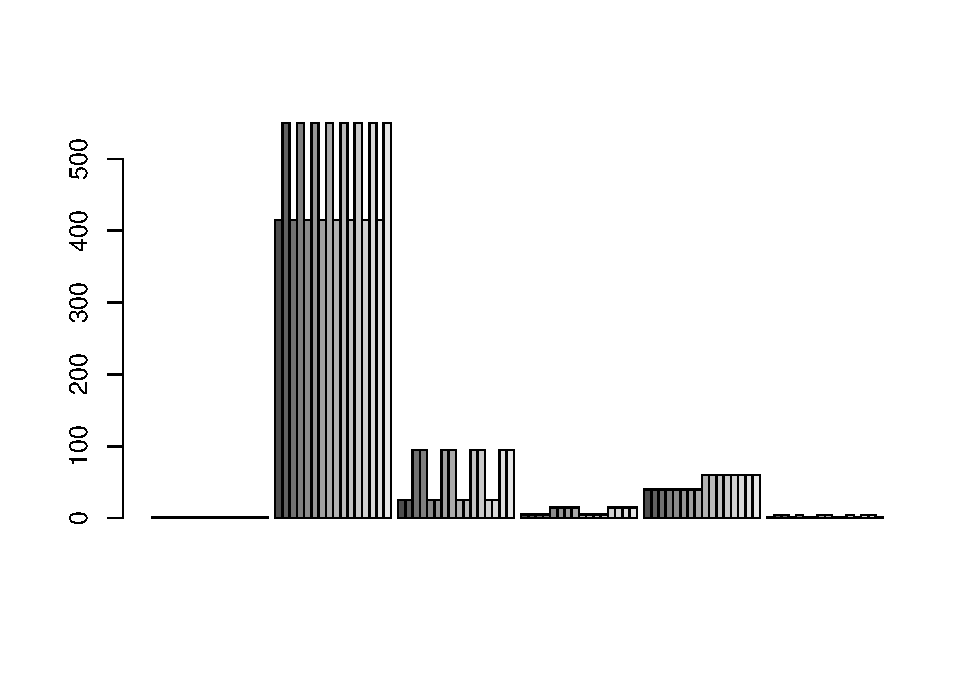
\includegraphics{Grupo13_Exercicio02_files/figure-latex/unnamed-chunk-4-1.pdf}

Dessa forma, vemos que a função de verossimilhança muda tanto em locação
como escala, pois valores grandes de \(\lambda\) alocam a distribuição
para direita, além de deixá-la mais achatada.

\begin{itemize}
\item
  \begin{enumerate}
  \def\labelenumi{\alph{enumi})}
  \setcounter{enumi}{2}
  \tightlist
  \item
    caso a resposta ao item b) seja afirmativa, encontre a escala na
    qual a função de verossimilhança mude somente em locação. Mostre
    graficamente.
  \end{enumerate}
\end{itemize}

\[\phi \propto \int \pi(\theta) d\theta = \int \theta^{-1/2} d\theta = 2\sqrt\theta  \propto
 \sqrt\theta \]

A equação acima expressa a chamada \emph{Lei de Jeffreys} que afirma que
a distribuição a priori para um único parâmetro \(\theta\) é
aproximadamente não informativa se tomada de modo proporcional à raiz
quadrada da Informação de Fisher de \(\theta\).

\begin{Shaded}
\begin{Highlighting}[]
\NormalTok{df }\SpecialCharTok{\%\textgreater{}\%}  \FunctionTok{ggplot}\NormalTok{(}\FunctionTok{aes}\NormalTok{(}\AttributeTok{x =} \FunctionTok{sqrt}\NormalTok{(theta))) }\SpecialCharTok{+}
  \FunctionTok{geom\_line}\NormalTok{(}\FunctionTok{aes}\NormalTok{(}\AttributeTok{y =} \FunctionTok{sqrt}\NormalTok{(L), }\AttributeTok{color =}\NormalTok{ lambda)) }\SpecialCharTok{+}
  \FunctionTok{geom\_line}\NormalTok{(}\FunctionTok{aes}\NormalTok{(}\AttributeTok{y =} \FunctionTok{dgamma}\NormalTok{(theta, }\DecValTok{1}\SpecialCharTok{/}\DecValTok{2}\NormalTok{, }\FloatTok{0.001}\NormalTok{), }\AttributeTok{linetype =} \StringTok{"Priori de Jeffreys"}\NormalTok{)) }\SpecialCharTok{+}
  \FunctionTok{labs}\NormalTok{(}\AttributeTok{color=} \FunctionTok{expression}\NormalTok{(lambda), }
       \AttributeTok{title =} \FunctionTok{expression}\NormalTok{(}\StringTok{"Verossimilhança normalizada de uma Poisson"}\SpecialCharTok{\textasciitilde{}}\NormalTok{(lambda)),}
       \AttributeTok{subtitle =} \StringTok{"Amostra aléatória com n=20"}\NormalTok{,}
       \AttributeTok{x =} \FunctionTok{expression}\NormalTok{(Phi),}
       \AttributeTok{y =} \FunctionTok{expression}\NormalTok{(}\FunctionTok{L}\NormalTok{(Phi))) }\SpecialCharTok{+}
  \FunctionTok{scale\_linetype\_manual}\NormalTok{(}\AttributeTok{name =} \StringTok{" "}\NormalTok{, }\AttributeTok{values =} \StringTok{"dotted"}\NormalTok{) }\SpecialCharTok{+}
  \FunctionTok{theme\_pubr}\NormalTok{()}
\end{Highlighting}
\end{Shaded}

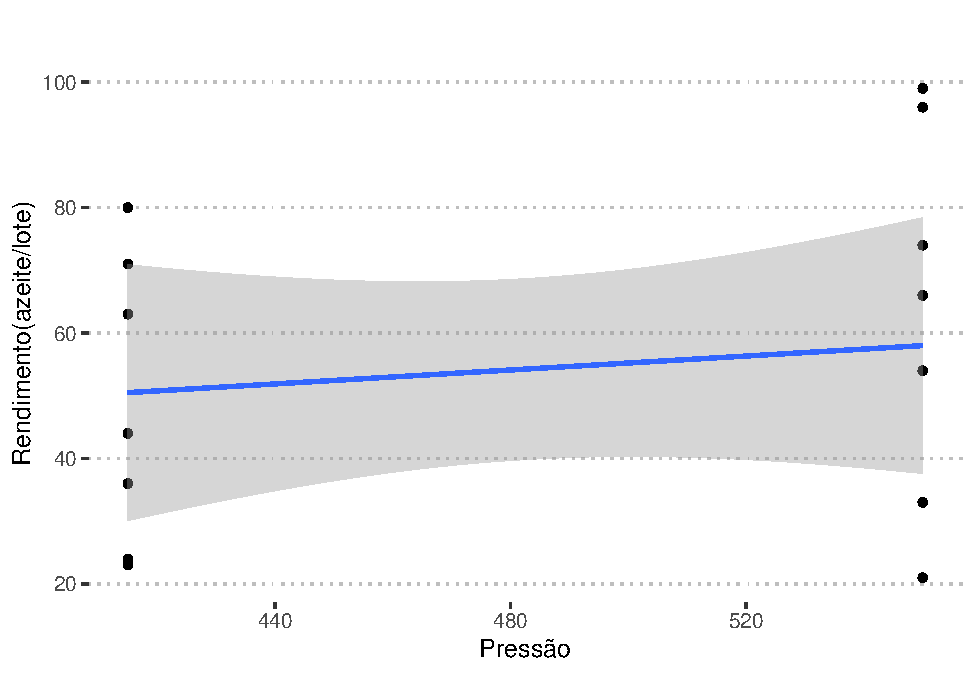
\includegraphics{Grupo13_Exercicio02_files/figure-latex/unnamed-chunk-5-1.pdf}

\end{document}
